% --------------------- EMPIRICAL RESULTS -----------------------------
\section{Empirical Results}
\label{sec:results}

\subsection{Prediction: accuracy is not enough}

Table~\ref{tab:acc} reports out-of-sample classification performance over 26 rebalancing events. The rule-book variables contain strong signal: every learned model has AUROC above 0.97, even 100 trading days before the effective date. However, accuracy alone gives the wrong investment ranking. The naive model that simply repeats last period's membership has the highest accuracy, 95.07\%, but predicts no changes and therefore cannot be traded.

\begin{table}[H]
\centering
\footnotesize
\begin{tabular}{lccccccc}
\toprule
Model & Acc. & Prec. & Sens. & Spec. & F & AUROC & Pred.\ changes \\
\midrule
\texttt{index\_lag1} & 0.9507 & 0.9208 & 0.9399 & 0.9565 & 0.9303 & 0.9446 & 0 \\
\midrule
GLM-100  & 0.9506 & 0.9292 & 0.9328 & 0.9605 & 0.9310 & 0.9789 & 63  \\
GLM-60   & 0.9497 & 0.9293 & 0.9298 & 0.9607 & 0.9296 & 0.9808 & 76  \\
GLM-30   & 0.9482 & 0.9259 & 0.9288 & 0.9589 & 0.9274 & 0.9797 & 93  \\
XGBB-30  & 0.9398 & 0.9316 & 0.9030 & 0.9613 & 0.9171 & 0.9812 & 174 \\
XGBB-60  & 0.9408 & 0.9331 & 0.9043 & 0.9621 & 0.9184 & 0.9817 & 165 \\
XGBC-30  & 0.9260 & 0.9208 & 0.8780 & 0.9548 & 0.8989 & 0.9812 & 271 \\
XGBC-60  & 0.9317 & 0.9318 & 0.8834 & 0.9609 & 0.9069 & 0.9817 & 247 \\
\bottomrule
\end{tabular}
\caption{\textbf{Out-of-sample prediction performance, 2010--2023.} Representative model-horizon combinations. ``Pred.\ changes'' is the total number of predicted additions plus deletions. XGBB is standard XGBoost; XGBC applies the conditional threshold in equation~(\ref{eq:cppt}).}
\label{tab:acc}
\end{table}

The conditional threshold does what it is designed to do. XGBC-30 reduces accuracy by 1.4 percentage points relative to XGBB-30, but increases predicted changes from 174 to 271. This is not a cosmetic difference: an index-event strategy earns nothing from correctly predicting that Equinor remains in the benchmark. It earns from the small set of names whose membership changes, and the model must create enough of those signals to diversify event risk.

\subsection{Active long--short overlays}

The active strategy confirms that prediction quality translates into investable return, but through two different channels. Table~\ref{tab:ff3} summarises monthly performance over the factor-test window. OSEBX earned 0.95\% per month with 4.23\% volatility. GLM-60 and GLM-100 produce the highest excess returns, but they do so with concentrated books and high volatility. XGBC-30 produces lower raw excess return, but is closer to the benchmark in beta and tracking error.

\begin{table}[H]
\centering
\footnotesize
\setlength{\tabcolsep}{3.5pt}
\begin{tabular}{lcccccccc}
\toprule
Portfolio & $R_p-R_b$ & $R_p$ & $\sigma_p$ & SR & $\alpha_{CAPM}$ & $\beta$ & TE$_{ann}$ & $\alpha_{FF3}$ \\
\midrule
OSEBX   & 0.0000 & 0.0095 & 0.0423 & 0.198 & 0.0002 & 1.015 & 0.000 & 0.001 \\
\midrule
GLM-60  & \textbf{0.0095} & 0.0190 & 0.0756 & 0.237 & 0.0139 & 0.497 & 0.260 & \textbf{0.013$^{**}$} \\
GLM-30  & 0.0034 & 0.0129 & 0.0511 & 0.231 & 0.0048 & 0.863 & 0.126 & \textbf{0.006$^{**}$} \\
XGBC-30 & 0.0017 & 0.0112 & 0.0441 & 0.229 & 0.0026 & 0.925 & 0.079 & \textbf{0.004$^{**}$} \\
GLM-100 & 0.0087 & 0.0182 & 0.0757 & 0.226 & 0.0133 & 0.468 & 0.267 & \textbf{0.013$^{**}$} \\
XGBB-30 & 0.0010 & 0.0105 & 0.0488 & 0.192 & 0.0016 & 0.954 & 0.106 & 0.003 \\
XGBC-60 & $-$0.0029 & 0.0066 & 0.0480 & 0.114 & $-$0.0004 & 0.729 & 0.138 & 0.001 \\
\bottomrule
\end{tabular}
\caption{\textbf{Active long--short overlays, monthly returns, January 2010--May 2022.} Alphas use OSEAX as the market proxy and Norwegian Fama--French factors. $^{**}$ denotes $p<0.05$.}
\label{tab:ff3}
\end{table}

\begin{figure}[H]
\centering
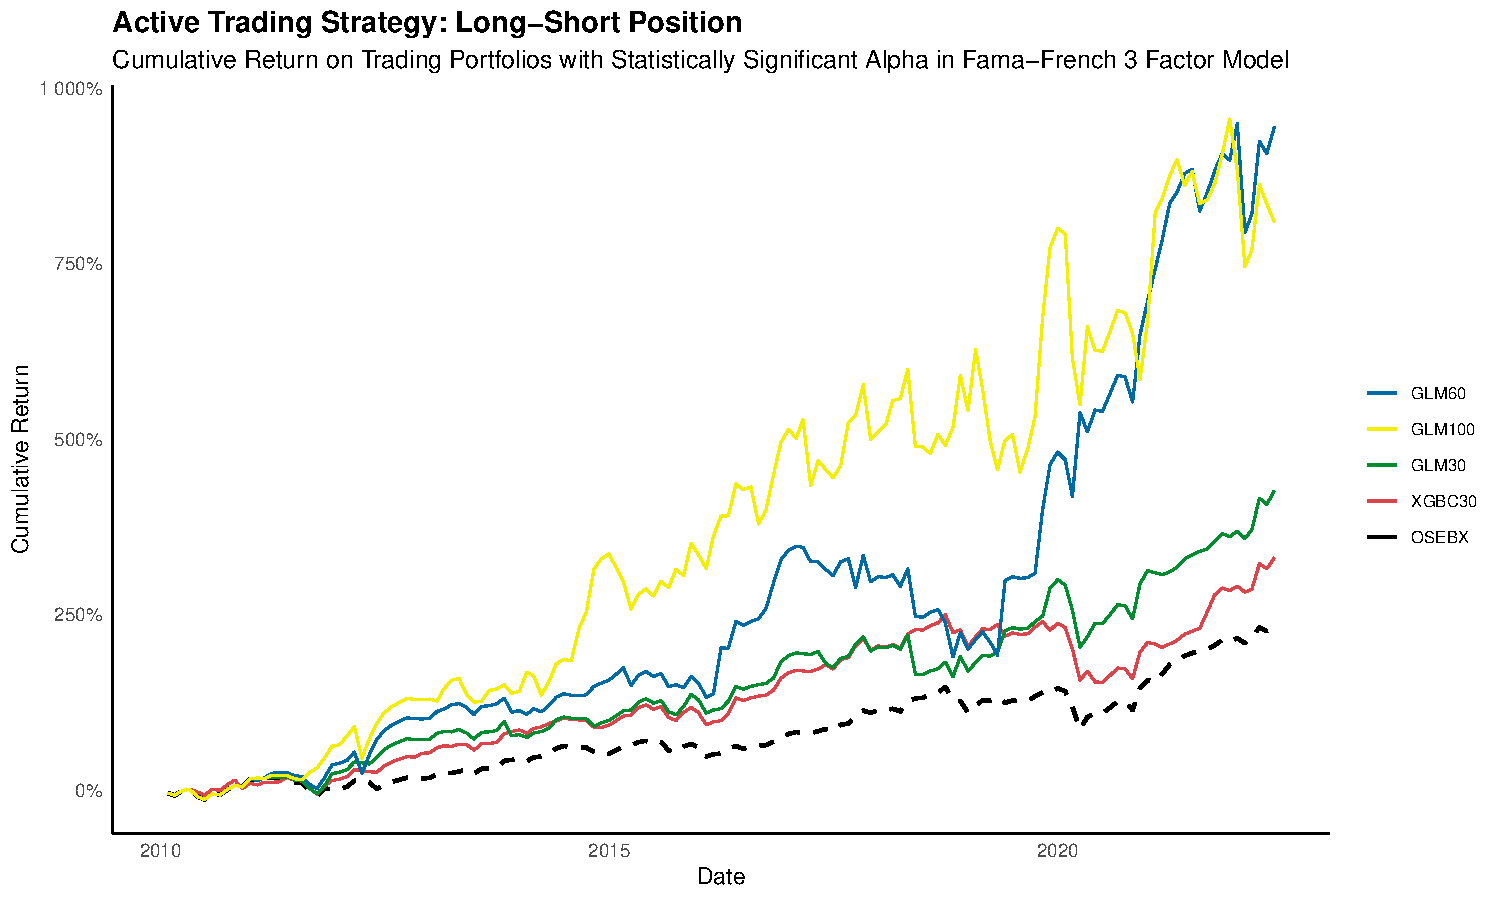
\includegraphics[width=0.78\linewidth]{images/trading_long_short.pdf}
\caption{\textbf{Cumulative active strategy returns.} Four active overlays with significant FF3 alpha compared with OSEBX. Initial capital is 1 NOK; transaction costs and short-borrow assumptions are included.}
\label{fig:cumret_active}
\end{figure}

For a discretionary active mandate, the GLM portfolios are attractive because they extract more return from fewer, cleaner signals. For a benchmarked mandate, the more important result is XGBC-30: it earns significant alpha while keeping annual tracking error below 8\% before any enhanced-index scaling. That lower active risk is what gives the signal capacity in the next test.

\subsection{Enhanced-index implementation}

The enhanced-index test is the stricter and more commercially relevant version. Each active overlay is scaled to the largest weight consistent with 2\% annual tracking error against OSEBX. This constraint sharply penalises concentrated portfolios: GLM-60 can only receive a 4.1\% active weight, while XGBC-30 can receive 22.1\%. After scaling, the ranking reverses. GLM still adds some raw return, but only XGBC-30 produces a positive FF3 alpha that is statistically distinguishable from zero at the 10\% level.

\begin{figure}[H]
\centering
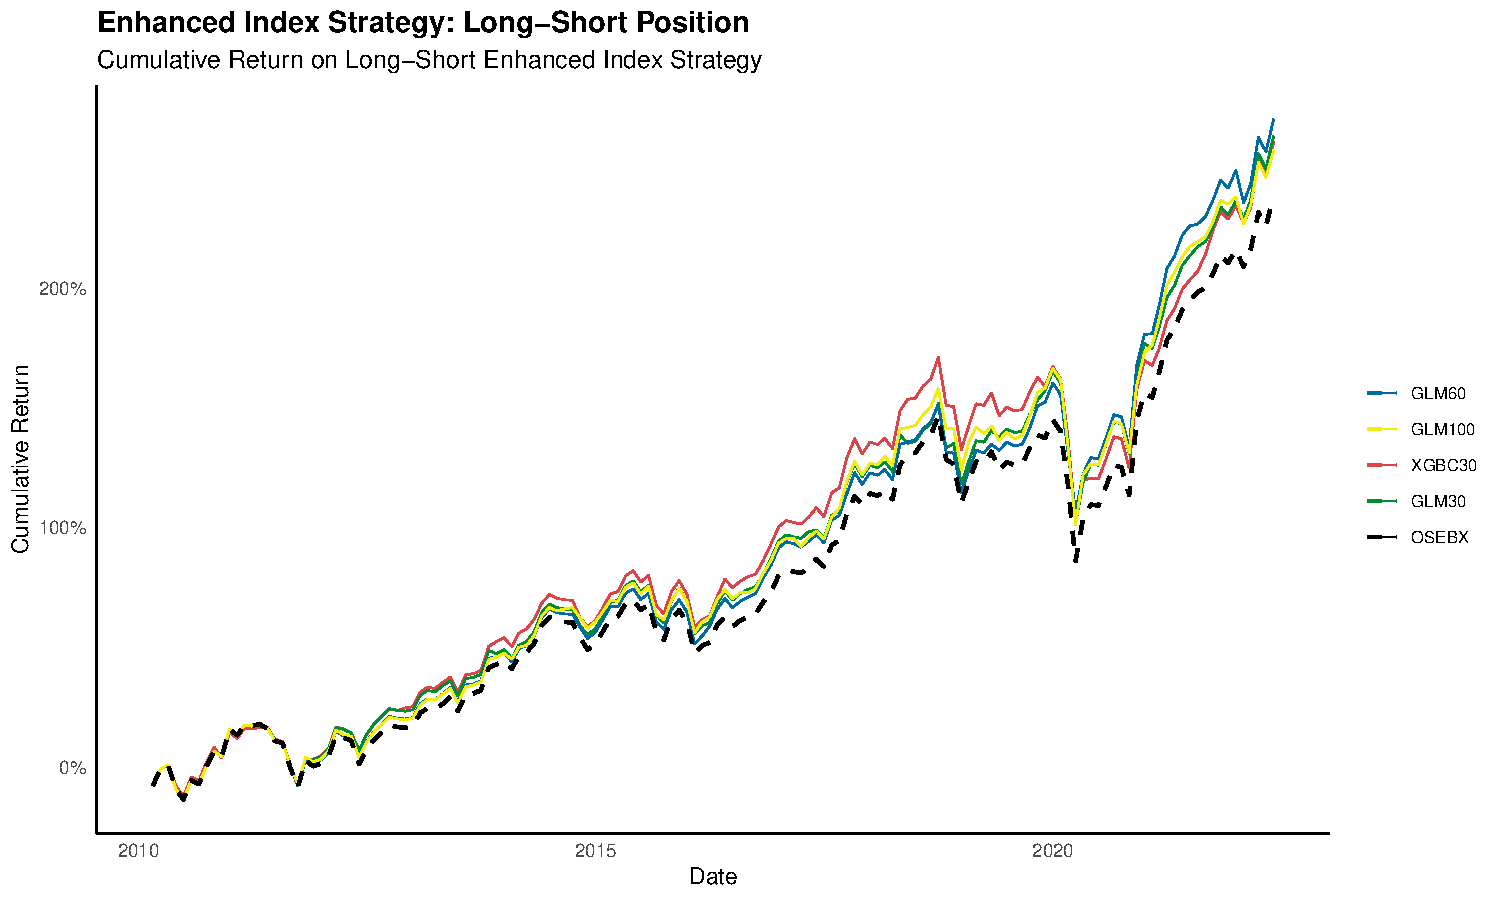
\includegraphics[width=0.78\linewidth]{images/enhanced_long_short.pdf}
\caption{\textbf{Enhanced-index portfolios.} Active overlays are combined with OSEBX and scaled to 2\% annual tracking error. XGBC-30 is the only long--short enhanced variant with significant FF3 alpha.}
\label{fig:cumret_enh}
\end{figure}

This is the practical finding. The same forecast that looks slightly worse in a classification table becomes the better product candidate once the portfolio is constrained like an enhanced-index fund. The threshold in equation~(\ref{eq:cppt}) is therefore not just a statistical tweak; it is a way to align the classifier with the economic objective.
